\chapter{Probability distributions}
Over all probability distributions used in this document, some of them are not usually part of the canonical background of a computer scientist.
We decided to present them in this appendix in order to have an overview for who has never seen them before.

\section{Beta distribution} \label{betad}
The Beta distribution is a family of continuous probability distributions.
It is defined in the range $[0, 1]$ and it has two parameters $\alpha,\beta > 0$.

Since $\alpha$ and $\beta$ are concentration parameters, they induce more and more sparsity as they approach the value of zero.
If $\alpha = \beta = 1$, the probability density function is uniform over $[0, 1]$.
As their values grow, the distribution tightens over its expectation.
All these observations can be seen empirically in Figure \ref{fig:betaparams}.

Due to its characteristics, it is suited to model probabilistic outcomes (for example, to describe how confident we are about the fact that a coin is loaded or not).

\begin{figure}[ht]
    \centering
    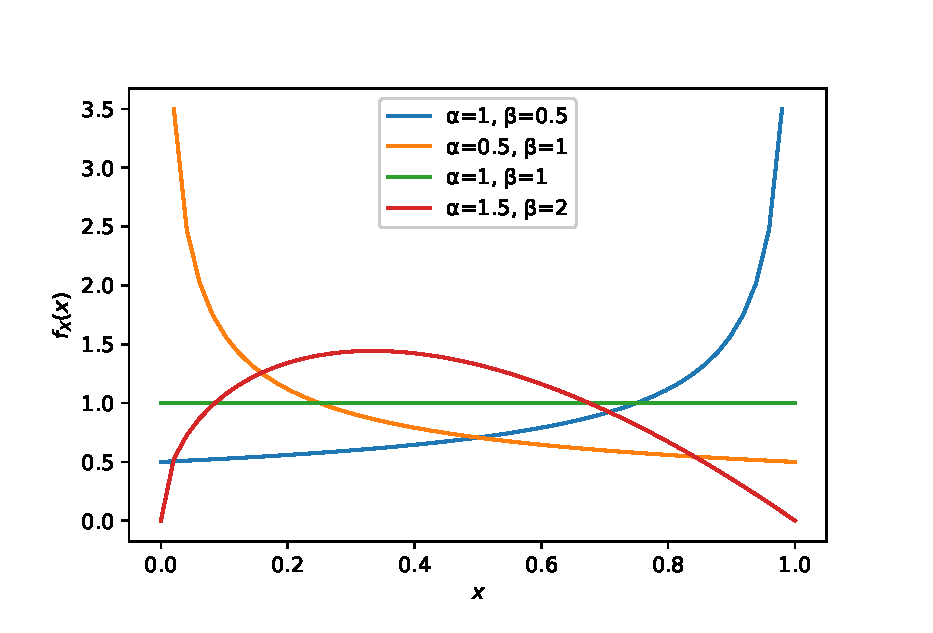
\includegraphics[width=0.7\textwidth]{images/beta}
    \caption{Example of the probability density function of a Beta distribution varying its parameters.}
    \label{fig:betaparams}
\end{figure}

\subsection{Probability density function}
Given a random variable $X \sim \mathit{Beta}(\alpha, \beta)$, the probability density function is defined as:
\[f_X(x) = \frac{1}{B(\alpha, \beta)}x^{\alpha - 1}(1-x)^{\beta - 1}\]
$\mathit{Beta}(\alpha, \beta)$ is the Beta function and it acts as a normalization constant to ensure that $\int_0^1 f_X(x) dx = 1$.

\section{Dirichlet distribution}
The Dirichlet distribution is a family of multivariate distributions.
It is parametrized by $K$ parameters, where $K$ is the number of random variables for which it is described.

It can be seen as a generalization of the Beta distribution: a Dirichlet distribution of 2 parameters $\mathit{Dir}(\alpha_1=a, \alpha_2=b)$ is a Beta distribution $\mathit{Beta}(\alpha=a, \beta=b)$.
All considerations and constraints about the parameters of the Beta distribution presented previously (Section \ref{betad}) still holds for the Dirichlet distribution.

\subsection{Probability density function}
Given a multivariate random variable $X \sim \mathit{Dir}(\alpha_1, \alpha_2, \dots, \alpha_K)$, the probability density function is defined as:

\[f_{X}(x_1, x_2, \dots, x_K; \alpha_1, \alpha_2, \dots, \alpha_K) = \frac{1}{B(\alpha_1, \alpha_2, \dots, \alpha_K)} \prod_{i=1}^{K} x_i^{\alpha_i - 1}\]

$\mathit{Beta}(\alpha_1, \alpha_2, \dots, \alpha_K)$ is the multivariate generalization of the Beta function presented in Section \ref{betad}.

Setting $\mathit{Dir}(\alpha) \coloneqq \mathit{Dir}(\alpha_1, \alpha_2, \dots, \alpha_n)$, a simplified notation of the probability density function is used:
\[f_{x}(x_1, x_2, \dots, x_K; \alpha) = \frac{1}{B(\alpha)} \prod_{i=1}^{K} x_i^{\alpha - 1}\]

The support is constrained by:
\begin{itemize}
    \item $x_i \in (0, 1), 1 \leq i \leq K $
    \item $\sum_{i=1}^K x_i = 1$
\end{itemize}

\subsection{Graphical intuition}
The support of a Dirichlet distribution with $K$ parameters lies in a $K-1$ simplex.
If $K=3$, the simplex is a triangle and can be represented graphically (see Figure \ref{fig:dirparams}).

All values of the probability density function $f_X(x_1, x_2, x_3): \Re^3 -> \Re$ are associated with a specific color given their intensity.
Bigger values in the probability density function are represented with lighter colors and vice versa.

Vertices of the simplex represent the situations in which $x = \begin{bmatrix}1 & 0 & 0 \end{bmatrix}$, $x = \begin{bmatrix}0 & 1 & 0 \end{bmatrix}$ or $x = \begin{bmatrix}0 & 0 & 1 \end{bmatrix}$.
If $x = \begin{bmatrix}\frac{1}{3} & \frac{1}{3} & \frac{1}{3} \end{bmatrix}$, we are at the center of the simplex.
Given an area of the triangle lighter than others, the probability of obtaining a vector in that interval during sampling is higher and vice versa.

Suppose we are in a supermarket and we are interested in the kind of purchases consumers make.
We define three categories: \say{food}, \say{technology} and \say{stationery}.
A strong preference over one category is represented modelling the probability density function with higher values towards one of the vertices.
Sampling from a Dirichlet distribution as the one represented in the left simplex in Figure \ref{fig:dirparams} will tend to give us users who do not have a strong preference over one category.
The opposite situation (for example, $\alpha_1=0.1, \, \alpha_2=0.1, \, \alpha_3=0.1$) will otherwise give us customers who strongly prefer one of the categories (for example. $x = \begin{bmatrix}0.8 & 0.15 & 0.05 \end{bmatrix}$) while users without propensities will be much rare.
Finally, if the probability density function is uniform over all the support (right simplex in Figure \ref{fig:dirparams}) there is no tendency of choosing a particular combination of categories over others.

\begin{figure}[ht]
    \centering
    \subfigure{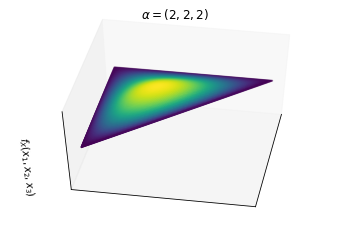
\includegraphics[width=0.5\textwidth]{images/dirichlet-1.png}}%
    \hfill
    \subfigure{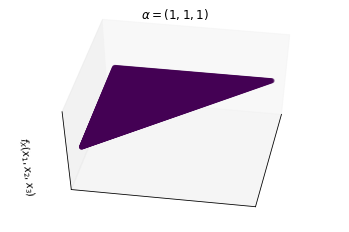
\includegraphics[width=0.5\textwidth]{images/dirichlet-2.png}}
    \caption{Example of the probability density function over a simplex of a Dirichlet distribution varying its three parameters $\alpha = (\alpha_1, \alpha_2, \alpha_3)$. The lighter the color, the higher the probability density function.}
    \label{fig:dirparams}
\end{figure}

\section{Categorial distribution}
The categorical distribution is a generalized Bernoulli distribution in the case of categorical random variables.

In the literature about Topic Modeling, it is wrongly used with the name of Multinomial distribution.
To keep the same notation as the papers in the bibliography, we will say that $X \sim \mathit{Mult}(p)$ means that X is distributed as Categorical.
Note that a Categorical distribution $\mathit{Mult}(p)$ is a special case of a Multinomial distribution $\mathit{Mult}(n, p)$ in which $n=1$.

Each $p_i$ of the parameter $p = (p_1, p_2, \dots, p_K)$ represents the probability of observing $i$ by sampling from the distribution.

\subsection{Probability mass function}
Given a random variable $X \in \mathit{Mult}(p)$, the probability mass function is defined as:
\[P(x == i) = p_i\]

\section{References}
The interested reader may refer to \cite{Gupta2011}, \cite{DBLP:journals/jmlr/BleiNJ03} and \cite{Seber2011} to use them as references.